El interés compuesto es un interés que se aplica no solo al capital inicial de una inversión o un préstamo, sino también a los intereses acumulados de periodos anteriores. En otras palabras, el interés compuesto implica ganar, o adeudar, intereses sobre los intereses.

El poder de la capitalización ayuda a que una suma de dinero crezca más rápido que si se calculara solo el interés simple sobre el capital. Y cuantos más periodos de capitalización, mayor será el crecimiento del interés compuesto. Para ahorros e inversiones, el interés compuesto es un aliado, ya que multiplica el dinero a un ritmo acelerado. Pero si se tienen deudas, la capitalización de los intereses que se deben puede dificultar cada vez más su pago.

El interés compuesto es conocido como "Interés sobre interés" (\textit{Interest on interest}).

El efecto de acumulación se vuelve especialmente poderoso sobre largos periodos de tiempo, a medida que la cantidad de intereses ganados se hace cada vez mayor.

\textit{El interés compuesto es la octava maravilla del mundo. Quien lo entiende, lo gana; quien no, lo paga.} - Albert Einstein.

\textbf{Variables}

\begin{itemize}
  \item \textbf{P}: \textit{Principal}. Monto inicial.
  \item \textbf{r}: \textit{Interest rate}. Tasa de interés.
  \item \textbf{n}: \textit{Number of periods}. Número o frecuencia de periodos de acumulación en un año.
  \item \textbf{t}: \textit{Time}. Tiempo transcurrido contabilisado en años.
  \item \textbf{A}: \textit{Amount}. Monto final total.
\end{itemize}

La ecuación \ref{equintsimple} sobre el interés simple, solo toma en cuenta el monto inicial. Sin embargo, el interés compuesto también considera el interés del periodo anterior. Por lo tanto, la parte de la ecuación que expresa el interés se repite.

\[
  1 + r
\]

Los periodos de acumulación se repiten. Debido a ello, se obtiene la siguiente expresión:

\[
  A = P(1 + r)(1 + r)
\]

Para múltiples periodos se obtiene lo siguiente:

\[
  A = P(1 + r)n
\]

El hecho de que $n$ sea un exponente, previamente en el interés simple era un factor multiplicador, hace que el interés compuesto crezca más rápido.

Para comparar los distintos intereses con las mismas métricas, se adopta una convención para que todos los intereses sean tratados, al menos en gran parte, como anuales. Y para incluir las distintas acumulaciones, estas se realizan respecto a cuantas se acumulan dentro de un año.

Suponiendo una longitud de un año de 365 días (año no bisiesto), algunos posibles valores de $n$ se muestran en la siguiente tabla:

\begin{table}
  \caption{Posibles frecuencias de acumulación}\label{tabfrcacm}
  \begin{center}
    \begin{tabular}{|c|c|}
      \hline
      \textbf{Frecuencia de acumulación} & \textbf{n} \\
      \hline
      Anual, un año, 12 meses & 1 \\
      \hline
      Semestral, medio año, 6 meses & 2 \\
      \hline
      Cuatrimestral, tercio de año, 4 meses & 3 \\
      \hline
      Trimestral, cuarto de año, 3 meses & 4 \\
      \hline
      Bimestral, sexto de año, 2 meses & 6 \\
      \hline
      Mensual, doceavo de año, 1 meses & 12 \\
      \hline
      Diario & 365 \\
      \hline
      Cada hora & 8 760 \\
      \hline
      Cada minuto & 525 6000 \\
      \hline
      Cada segundo & 31 536 000 \\
      \hline
    \end{tabular}
  \end{center}
\end{table}


Como se puede observar en la tabla \ref{tabfrcacm}, mientras más frecuente es la acumulación más grande es el valor de $n$. Lo cual resulta en un mayor valor acumulado.

Hay que considerar que el interés se toma en cuenta para cada acumulación, esto es el interés en cada periodo. lo cual se representa de la siguiente forma:

\[\boxed{
  \dfrac{r}{n}
}\]

La cantidad de años transcurridos también es afectada por la cantidad acumulaciones en esos años. Dado que se considera los años y los periodos por año, multiplicándolos se obtiene la cantidad total de periodos. Esto resulta en lo siguiente:

\[\boxed{
  nt
}\]

Teniendo en cuenta cada una de las variables y como se relacionan, se obtiene una fórmula que describe el interés compuesto.

\begin{listequbox}
  {A = P\left(1+\dfrac{r}{n}\right)^{\displaystyle nt}}{equintcmp}{Interés compuesto}
\end{listequbox}

Para observar como se desarrolla el interés compuesto se utilizará el siguiente ejemplo: Se realiza una inversión inicial de \$100 con una tasa de interés del 10\% con una acumulación mensual durante 5 años. El aumento del monto total se muestra en la siguiente tabla:

\begin{table}[H]
  \center
  \caption{Evolución interés compuesto}\label{tabintcomp}
  \begin{tabular}{|c|c|}
    \hline
    \textbf{n} & \textbf{Monto total} \\
    \hline
    0 & 100 \\
    \hline
    1 & 110.47 \\
    \hline
    2 & 122.04 \\
    \hline
    3 & 134.82 \\
    \hline
    4 & 148.94 \\
    \hline
    5 & 164.53 \\
    \hline
  \end{tabular}
\end{table}

Comparando las tablas \ref{tabintsimple} y \ref{tabintcomp}, la diferencia entre el monto final de 150, del interés simple, y 164.53, del interés compuesto, es de 14.53. Lo cual representa, para montos más grandes, una diferencia muy significativa.

A continuación se muestra una representación gráfica del crecimiento del interés compuesto:

\begin{tikzpicture}
  \begin{axis}[
    xmin=0,xmax=6,
    xtick={0,1,2,3,4,5},xticklabels={0,1,2,3,4,$t$},
    ymin=90,ymax=170,
    ytick={100,164.53},yticklabels={\text{Inicial (P)},\text{Final (A)}},
    xlabel={\text{Tiempo (años)}},
    ylabel={\text{Monto total}},
    axis lines=left
    ]
    \addplot[color=blue,domain=0:5,thick]{100*((1+(0.1/12))^(12*x))};

    \draw[black!50,dashed] (axis cs:5,0) -- (axis cs:5,164.53);
    \draw[black!50,dashed] (axis cs:0,164.53) -- (axis cs:5,164.53);
  \end{axis}
\end{tikzpicture}

En un inicio el crecimiento es muy marcado, sin embargo, cuando $t$ toma valores muy grandes imcrementa de manera cada vez más lenta. La curva se vuelve más empinada. Considerando un periodo de 30 años, la gráfica es la siguiente:

\begin{grafica}[H]
\center
\begin{tikzpicture}
  \begin{axis}[
    xmin=0,xmax=32,
    xtick={0,5,10,15,20,25,30},xticklabels={0,5,10,15,20,25,$t$},
    ymin=90,ymax=2100,
    ytick={100,1983.74},yticklabels={\text{Inicial (P)},\text{Final (A)}},
    xlabel={\text{Tiempo (años)}},
    ylabel={\text{Monto total}},
    legend style={at={(0.6,0.85)},inner sep=9pt},
    axis lines=left
    ]
    \addplot[color=blue,domain=0:30,thick]{100*((1+(0.1/12))^(12*x))};
    \addlegendentry{$A = P\left(1+\dfrac{r}{n}\right)^{\displaystyle nt}$}

    \draw[black!50,dashed] (axis cs:30,0) -- (axis cs:30,1983.74);
    \draw[black!50,dashed] (axis cs:0,1983.74) -- (axis cs:30,1983.74);
  \end{axis}
\end{tikzpicture}
\caption{Crecimiento interés compuesto}
\end{grafica}

El poder el interés compuesto radica en el tiempo, el recurso más valioso que hay. Mientras más pronto se ahorre, más se tendrá en el futuro.

A continuación se muestra una comparación entre interés simple y compuesto, tomando los ejemplos presentados anteriormente.

\begin{grafica}[H]
\center
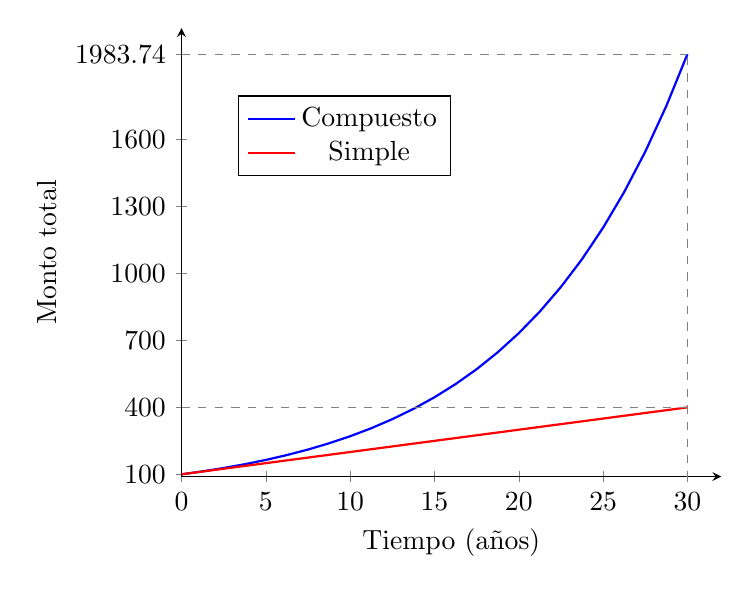
\begin{tikzpicture}
  \begin{axis}[
    xmin=0,xmax=32,
    xtick={0,5,10,15,20,25,30},xticklabels={0,5,10,15,20,25,30},
    ymin=90,ymax=2100,
    ytick={100,400,700,1000,1300,1600,1983.74},yticklabels={100,400,700,1000,1300,1600,1983.74},
    xlabel={\text{Tiempo (años)}},
    ylabel={\text{Monto total}},
    legend style={at={(0.5,0.85)}},
    axis lines=left
    ]
    \addplot[color=blue,domain=0:30,thick]{100*((1+(0.1/12))^(12*x))};
    \addlegendentry{\text{Compuesto}}
    \addplot[color=red,domain=0:30,thick]{100*(1+(x*0.1))};
    \addlegendentry{\text{Simple}}

    \draw[black!50,dashed] (axis cs:30,0) -- (axis cs:30,1983.74);
    \draw[black!50,dashed] (axis cs:0,400) -- (axis cs:30,400);
    \draw[black!50,dashed] (axis cs:0,1983.74) -- (axis cs:30,1983.74);
  \end{axis}
\end{tikzpicture}
\caption{Comparación interés simple y compuesto}
\end{grafica}

Como se puede observar, el rendimiento del interés compuesto es muy superior al del interés simple. Principalmente al factor exponencial del interés compuesto, a diferencia de la naturaleza lineal del interés simple.
